\section{Evaluation}

The present section aims at evaluating the behavior of the \schim on
the target platform, its overhead and benefits.  First, in subsection
\ref{subsection:considered-architecture}, we review our experimental
setup. Thereafter, we assess the overhead introduced by the \schim in
Section~\ref{subsec:platform-capabilities-and-performance-degradation}.
Section \ref{sec:feedback-pressure} explores the impact of the PL-to-PS feedback
on the control and the performance.
In Section~\ref{subsec:internal-behaviour-of-schim}, an in-depth analysis
of the \schim's behavior is presented. Finally, an evaluation of the
temporal behavior of a set of real-world benchmarks operating through
the \schim is provided in Section~\ref{subsec:isolation}.


\subsection{Experimental Setup}
\label{subsection:considered-architecture}
The \schim has been evaluated using synthetic benchmarks (or
\emph{Memory Bombs}), real benchmarks selected from the San Diego
Vision Benchmark Suite (SD-VBS)~\cite{SD-VBS} and a combination of
the two. Specifically, seven memory-intensive benchmarks have
been selected, i.e. \emph{stitch}, \emph{texture synthesis},
\emph{disparity}, \emph{tracking}, \emph{localization}, \emph{mser}
and \emph{sift}. For our runs we have considered all the intermediate
input sizes ranging from SQCIF (128$\times$196 pixels) to VGA
(640$\times$480 pixels). When running any benchmark, we use the cache
coloring mechanism implemented in the Jailhouse
hypervisor~\cite{determ_virt} to partition the LLC evenly amongst the
4 cores and to prevent our measurements to be affected by inter-core
cache interference. As a result, each benchmark operates on 1/4 of the
total cache space---256~KB. As extensively discussed
in~\cite{bounding_rtas14, palloc_rtas14}, it is also important to
avoid inter-core DRAM bank conflicts, which can cause the arbitrary
reordering of transactions originating from different cores. This is
accomplished by (1) configuring the DRAM controller to disable DRAM
bank interleaving; and (2) by performing static cache
bleaching~\cite{gracioli2019designing, PLIM20} at the \schim's output
to re-compact accesses to colored pages into contiguous DRAM
accesses. In this platform, there are a total of 16 DRAM banks of
256~MB each. Thanks to bleaching, we are able to assign the full size
of 4 banks (i.e., 1~GB) to each core, instead of being restricted
to only 1/4 of that due to non-overlapping color and bank address
bits.

%  \todo[inline]{RM: this part is a bit redundant with the implementation section. We can remove this seciton and only keep the description of the routes we are gonna test. See above}
%    The COTS platform used for the following set of experiments, the Xilinx ZCU102 development board, features four cores which, with the LLC, composed the cores cluster. While the \schim can be configured to handle many more masters, in the present set of experiments, only the cores composing this cluster competes for main memory access. Consequently, the \schim module has been configured with four queues (one for each master) as shown in Figure \ref{fig:MemorEDF_module_schema}. Following the discussion in section \ref{sec:pl-to-ps-feedback}, \schim has been configured with two slave ports. Finally, the frequency of the PL side has been pushed to 250~MHz.

%    \todo[inline]{RM: The paragraph below to go into experimental setup}
To evaluate the capabilities of the \schim, two memory routes for
the traffic generated by the cores are compared. The first serves
as baselines, whereas, the last one is the one under analysis and
involves the \schim module.  The first path consists in the cores
directly accessing the main memory. As illustrated in
\fig{fig:PS-PL-diagram}, the traffic simply goes through the
\emph{Main Interconnect} before arriving at the DDR controller. This
path is referred to as the \emph{normal route}.
%In the second path,
%traffic is routed through the PL but without being subject to
%scheduling. In this case, a simple one-to-one connection between one
%of the HPM ports and the HPS port is programmed in the PL. No other
%manipulation on the traversing memory transactions is performed inside
%the PL; we refer to this case as the \emph{simple loop-back}.
%Finally,
Secondly, we consider the case where the \schim module is deployed and in
use to schedule memory traffic generated by the CPUs in the PL. Cores
0 and 1 target HPM1 aperture, while cores 2 and 3 target HPM2. In our
analysis, \schim is used in all the available modes, \replace{i.e., FP, TDMA
and TS.}{i.e., FP and TDMA.}

\subsection{Platform Capabilities and performance degradation}
\label{subsec:platform-capabilities-and-performance-degradation}
Intuitively and as discussed in~\cite{PLIM20}, redirecting the traffic
coming from the cores to the PL side incurs a performance hit. In
spite of the lower frequency at which the \schim operates (250~MHz),
the theoretical throughput when using both the HPM lanes should be
around 8~GB/s. We observe however that the achievable throughput
through the HPM ports is a fraction of that due to what appears to be
PS-side internal throttling. For the sake of completeness, we quantify
in \fig{fig:bandwidth_comparison} the maximum bandwidth achieved
through the PL --- and hence through the \schim. But it is important
to remember that the absolute figures are strictly platforms
dependent.

In \fig{fig:bandwidth_comparison}, we have computed the throughput of
one \emph{core under analysis}, here core 0 (noted $C_{0}$) when a
synthetic memory-intensive application is deployed on an increasing
number of cores denoted with the same notation. The first bar cluster
(``Normal'') refers to the throughput measured via the normal
route. The other three clusters capture the observed bandwidth when
traffic is routed through and managed by the \schim.
One cluster is provided for each of the implemented memory scheduling policies,
namely --- from left to right --- \replace{FP, TDMA, and TS}{FP and TDMA}.
As expected, there is a sharp reduction (around 75\%) in terms of absolute
bandwidth. Importantly, however, two aspects need to be
highlighted. First, the bandwidth achieved through the \schim is still
remarkably high and allows studying the behavior of realistic workload
under custom memory scheduling policies, which is the main goal of
this research. Second, it emerges that the implemented FP and TDMA
policies are capable of protecting the core under analysis from
inter-core interference, while this is not the case when going through
the normal route
\removed{
, nor when using the TS policy at the \schim.
}


%% for each
%% of the aforementioned paths under all the possible levels of
%% contention. The result of this experiment is display in
%% \fig{fig:bandwidth_comparison}.

%% From , one can observe that in general,
%% the throughput experienced by the core under analysis (i.e., $C_{0}$)
%% is high and that, regardless of the contention level on the normal
%% route, the bandwidth remains high. As mentioned earlier, redirecting
%% the cores' traffic through the PL side has a cost. In fact, in the
%% case with no contention (the left-most bar cluster), the bandwidth
%% experienced by $C_{0}$ when going through the simple loop-back, is
%% reduced by around 75\% compared to the normal route.  Looking at the
%% left-most bar cluster, one can also observe the overhead introduced by
%% having the presence of the \schim on the memory loop-back. The
%% additional drop in bandwidth is approximately 185~MBps.  While the
%% throughput is larger in the case of the \emph{simple loop-back}, it
%% also drops linearly as soon as the contention level increases.  On the
%% other hand, the \schim manages to preserve the same bandwidth, with
%% negligible interference being observed in the most challenging
%% scenario (the right-most bar cluster). In other words, the \schim
%% guarantees performance isolation between the cores with respect to the
%% bus usage.

\begin{figure}
  \centering
  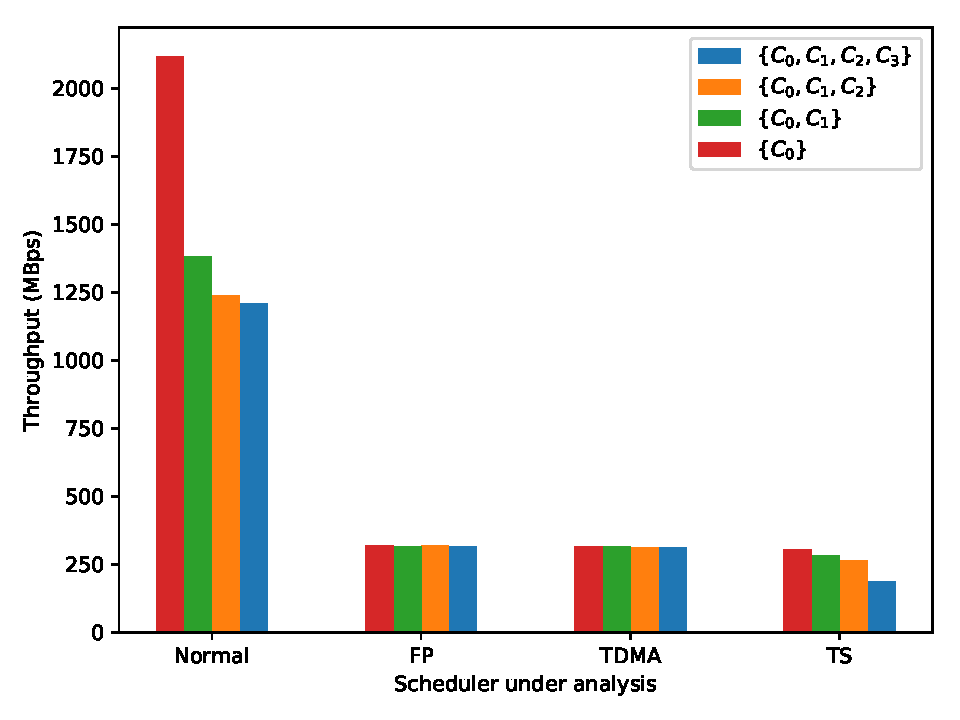
\includegraphics[scale=0.45]{images/bw_comparisons.pdf}
  \caption{Bandwidth in MBps for different path under increasing set of cores contending.}
  \label{fig:bandwidth_comparison}
\end{figure}

\subsection{PL-to-PS feedback performance impact}
\label{sec:feedback-pressure}
\begin{figure}[]
  \centering
  \begin{subfigure}{0.9\textwidth}
    \centering
    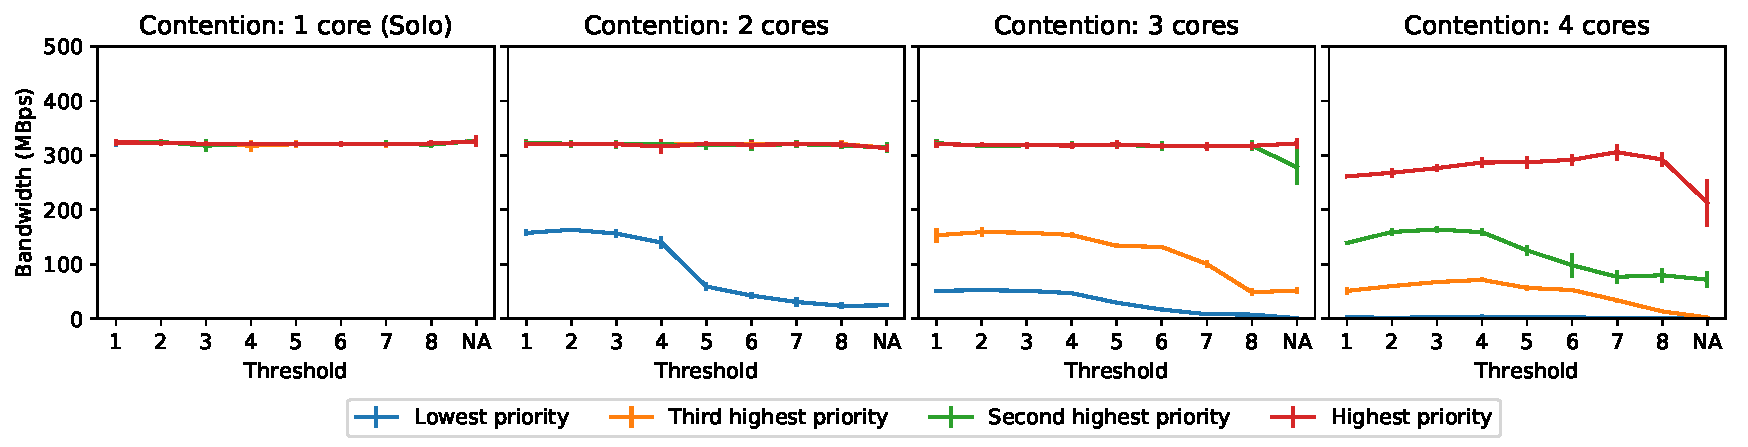
\includegraphics[scale=0.4]{images/fp.pdf}
    \caption{Threshold-Bandwidth relationship curves for the FP scheduler}
    \label{fig:threshold_fp}
  \end{subfigure}
  \hfill
  \begin{subfigure}{0.9\textwidth}
    \centering
    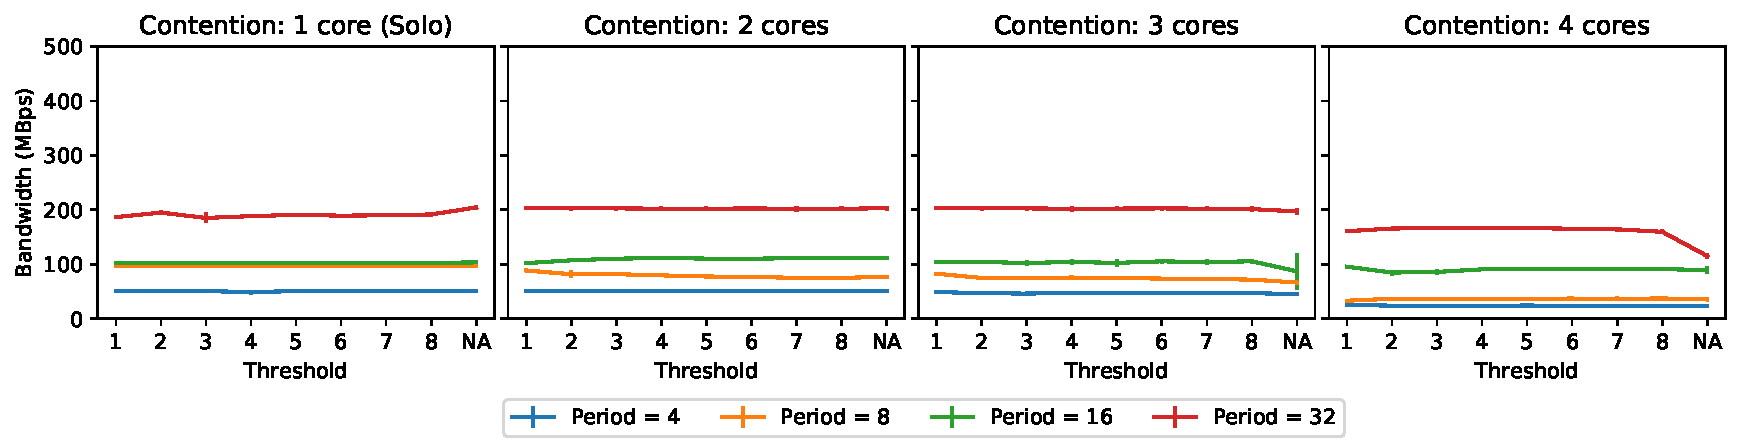
\includegraphics[scale=0.4]{images/tdma.pdf}
    \caption{Threshold-Bandwidth relationship curves for the TDMA scheduler}
    \label{fig:threshold_tdma}
  \end{subfigure}
%  \begin{comment}
%  \hfill
%  \begin{subfigure}{0.9\textwidth}
%    \centering
%    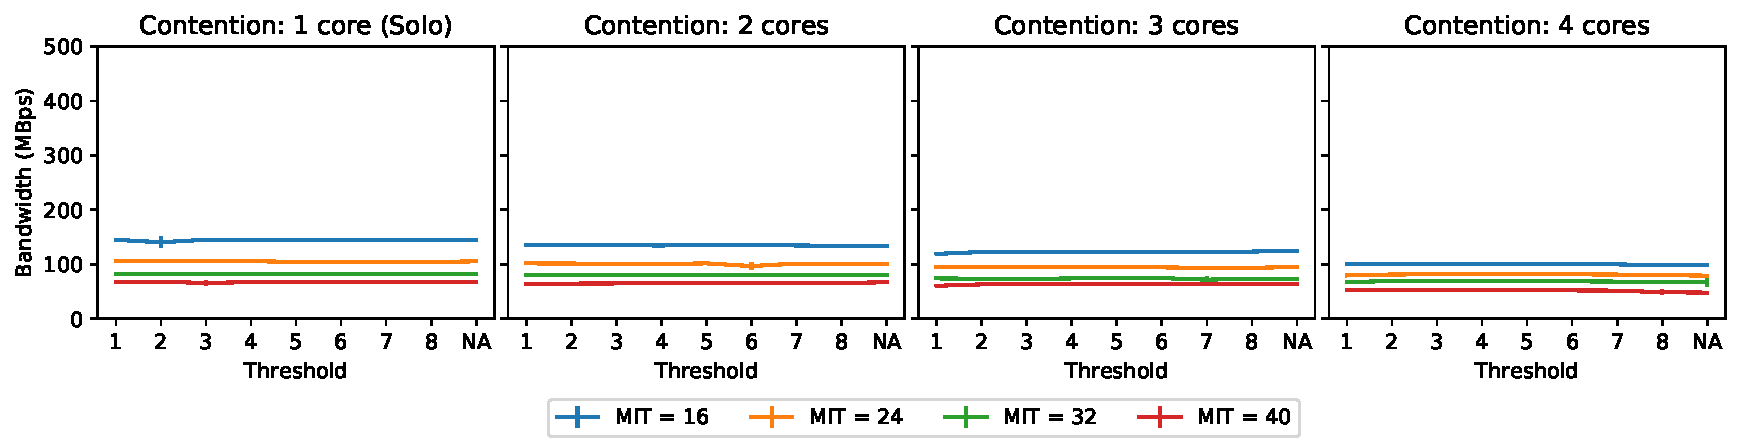
\includegraphics[scale=0.4]{images/ts.pdf}
%    \caption{Threshold-Bandwidth relationship curves for the TS scheduler}
%    \label{fig:threshold_ts}
%  \end{subfigure}
%\end{comment}
\textcolor{red}{TS subfigure removed}
  \caption{Figures showing the impact of the threshold in use on the final bandwidth experinced by the cores for the offered schedulers}
  \label{fig:schim_threshold}
\end{figure}
As mentioned in Section \ref{sec:pl-to-ps-feedback}, the PL-to-PS feedback enables
\schim to regulate the HPM ports buffer occupancy to prevent head-of-line blocking.
Since this feedback directly throttles the desired core, the selection of an adequate
threshold is important to preserve the balance between control and performance.
Therefore, in Figure \ref{fig:schim_threshold}, we have explored the sensitivity
to the threshold for each of the proposed schedulers under different levels of contention.
The thresholds in use range from 1 to 8 and even include the case where the feedback mechanism is disabled
(noted \emph{NA}). The contention is created by up to four co-running cores emitting
write transactions. For each parameter applied to a scheduler (i.e., fixed
priority, TDMA slot or MIT), the co-running cores are assigned the most
demanding parameters available (i.e., the highest priority for FP, the biggest TDMA
slot or the smallest MIT).

In the case of the FP scheduler (Figure \ref{fig:threshold_fp}), one can observe
that when running alone, the threshold has no influence on the throughput.
However, as soon as co-runners are added, the cores start to experience a
decrease in throughput.
Figure \ref{fig:threshold_tdma} shows that the TDMA scheduler is, with respect to the throughput, not impacted considerably by the threshold. Globally, the
scheduler manages to preserve a constant throughput regardless of the contention
and the assigned slot.
\removed{
Similarly, the TS scheduler is barely impacted by the choice of the threshold as
displayed in Figure \ref{fig:threshold_ts}.
}

Nonetheless, under high
contention, one can observe that the throughput of each core is affected.
The fourth inset of Figure \ref{fig:threshold_fp} and \ref{fig:threshold_tdma}
illustrate the importance of the threshold and the PL-to-PL feedback mechanism as a
a considerable drop of throughput can be observed for the highest priority of FP
and for a TDMA period of 32.

Considering these experiments, setting the threshold to four for all the schedulers
seems to bring the best trade-off between control and performance. However, this
value cannot be blindly applied to all cases as this experiment is performed for
a sequential and contiguous access pattern.

\subsection{Internal Behaviour of SchIM}
\label{subsec:internal-behaviour-of-schim}
The next objective is to verify the correct behavior of the schedulers
at the granularity of a clock cycle by observing the inputs,
the outputs and the internal signals and registers of the \schim
module. This is made possible thanks to the \emph{Integrated Logic
  Analyzer} (or ILA) provided by Xilinx \cite{Xilinx-ILA}. The latter
IP can be directly implemented on the PL side, alongside the \schim,
and is able to probe the signals and to store them in a local
memory. For this experiment, a group of relevant internal signals have
been probed and captured during a window of 16384 contiguous clock
cycles. Then, the information has been extracted by post-processing
the data. To characterize the behavior of the three different
policies, the ILA has been instrumented to collect (i) the amount of
transactions being buffered in the queues at each clock cycle
\replace{(inset 1 in \fig{fig:schim_behaviour_fp}, \fig{fig:schim_behaviour_tdma}, and
\fig{fig:schim_behaviour_mg}),}{(inset 1 in \fig{fig:schim_behaviour_fp} and \fig{fig:schim_behaviour_tdma})}
(ii) the rate at which queues receive
new transactions from the cores cluster
\replace{(inset 2 in \fig{fig:schim_behaviour_fp}, \fig{fig:schim_behaviour_tdma}, and
\fig{fig:schim_behaviour_mg}),}{(inset 2 in \fig{fig:schim_behaviour_fp} and \fig{fig:schim_behaviour_tdma})}
 and (iii) the queues ID of each
transaction forwarded by the \schim module
\replace{(inset 3 in \fig{fig:schim_behaviour_fp}, \fig{fig:schim_behaviour_tdma}, and
\fig{fig:schim_behaviour_mg}).}{(inset 3 in \fig{fig:schim_behaviour_fp} and \fig{fig:schim_behaviour_tdma}).}

For the Fixed Priority trace snapshot displayed in
\fig{fig:schim_behaviour_fp}, the following strict priority ordering
has been considered: $C_{0} \succ C_{1} \succ C_{2} \succ C_{3}$ where
the $\succ$ operator means that the left argument has a strictly
higher priority than the right argument. In this experiment, a
regulation threshold of 3 for each core has been used.  As emphasized
by the inset 2 in \fig{fig:schim_behaviour_fp}, the FP scheduler is
able to prioritize the traffic of one core at the expense of the
others according to the priorities assignment. Furthermore, one can
observe that the rate at which the queues receive new transactions
from their associated core is proportional to the priority place in
the priority ordering.  Finally, the third inset in
\fig{fig:schim_behaviour_fp} confirms the correct behavior of the FP
policy.%, with the higher the core's priority, the higher the transaction density at the output of \schim is.
%Thanks to the heat map, one can clearly see that the cores
%with the highest priority also feature the highest density of
%transactions at the output of the \schim.
One can see that the cores with the highest priority also feature the
highest density of transactions at the output of the \schim.

The trace snapshot displayed in \fig{fig:schim_behaviour_tdma} has
been obtained by configuring the \schim module in TDMA mode. For the
sake of clarity, a slot of 256 clock cycles has been set for each
core. Besides, the threshold of each core has been set to 4 to
create sharp transitions.  The insets 2 and 3 of
\fig{fig:schim_behaviour_tdma} clearly show the behavior expected
from a TDMA schedule. In fact, one can clearly see in the latter that
transactions originating from one core are only being repeated out of
the \schim module during a well-defined and periodic time slot of 256 clock cycles. In the inset 2 of \fig{fig:schim_behaviour_tdma}, we can
observe a similar pattern, with transactions arriving only during the
TDMA slot associated with their queue (and indirectly core). Globally,
the rate at which queues receive transactions is steady and constant.
\removed{
The trace snapshot for the TS policy has been obtained with an MIT of
160 clock cycles for each core. Similar to the TDMA experiment, such
period has been set arbitrarily in order to improve the clarity of the
trace snapshot displayed in \fig{fig:schim_behaviour_mg}. Thanks to
the inset 3 in \fig{fig:schim_behaviour_mg}, we can see that under a significant traffic load, the TS mode of the \schim is able to shape
the output traffic. Roughly, the same pattern can be observed in the inset
2 of \fig{fig:schim_behaviour_mg}. However, there is an exception.
In both the second and the third insets, queue 3 (and indirectly core 3)
clearly violates the pattern expected from the TS scheduler. This transaction
leakage is due to a malfunction in the TS scheduler design.
}

%First, one queue can receive more than one transaction. This is due to
%the coarseness of the FIQ feedback regulation. Secondly, some queues
%seem to be prioritized. This can be explained by the fact that in the
%TS scheduler implementation break ties between valid ready transactions
%using a FP policy. In this experiment, since the \schim module is constantly under pressure, there are always ties between the queues and FP is frequently applied.
    \begin{figure}[t]
      \centering
      \begin{subfigure}{0.45\textwidth}
        \centering
        % include first image
        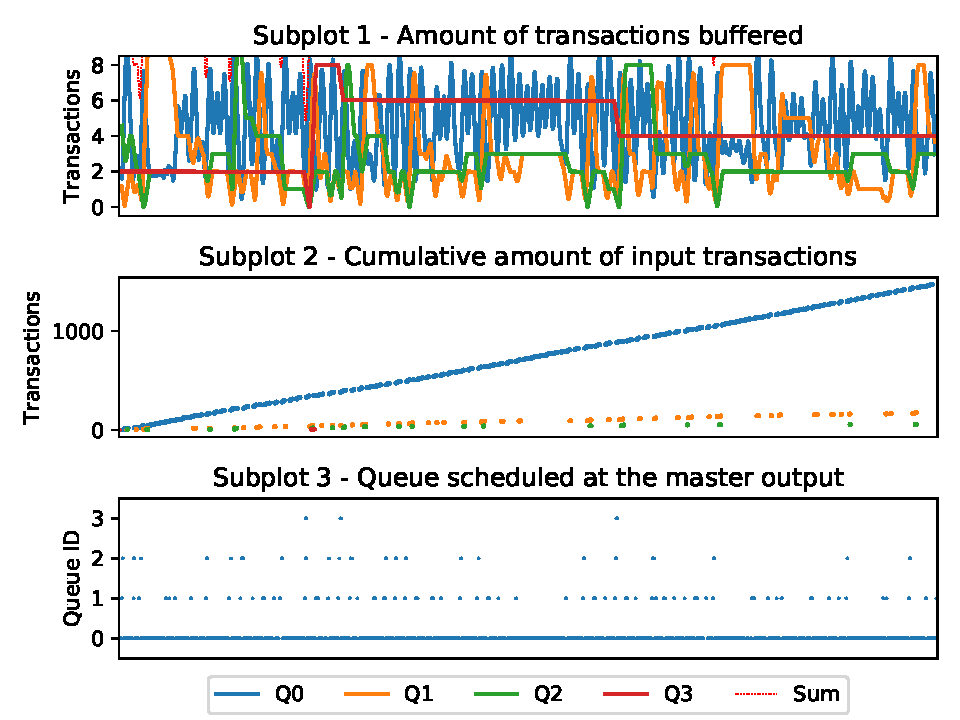
\includegraphics[scale=0.45]{images/SchIM_FP_buffering.pdf}
        \caption{FP with ordering $C_{0} \succ C_{1} \succ C_{2} \succ C_{3}$}
        \label{fig:schim_behaviour_fp}
      \end{subfigure}
      \hfill
      \begin{subfigure}{0.45\textwidth}
        \centering
        % include second image
        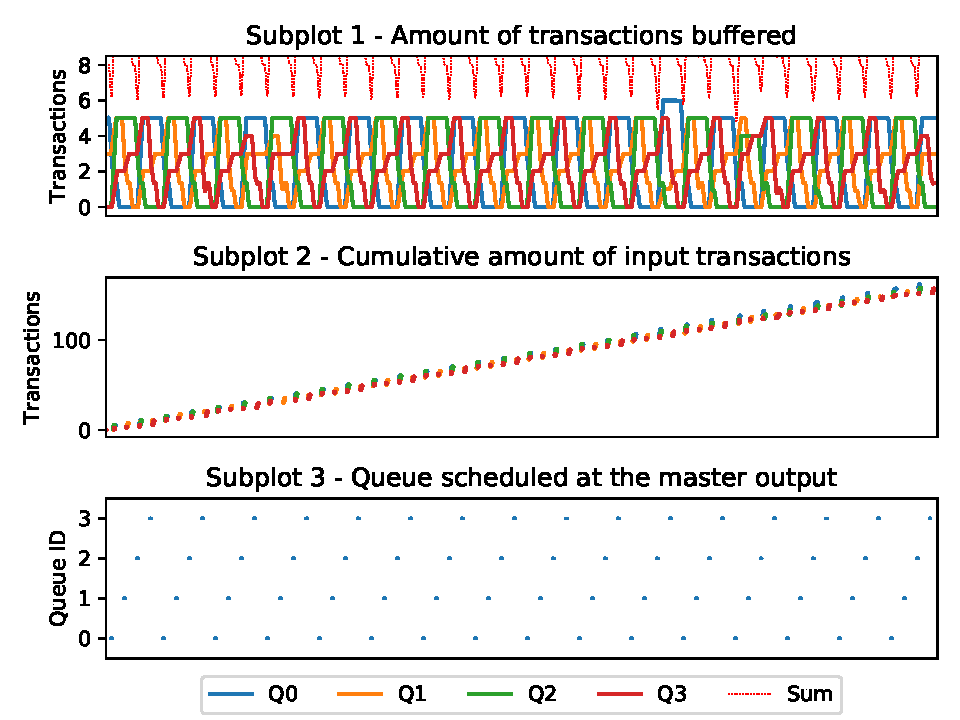
\includegraphics[scale=0.45]{images/SchIM_TDMA_buffering.pdf}
        \caption{TDMA with slots of 256 clock cycles}
        \label{fig:schim_behaviour_tdma}
      \end{subfigure}
      \hfill
      \begin{subfigure}{0.45\textwidth}
  %      \centering
  %      % include second image
  %      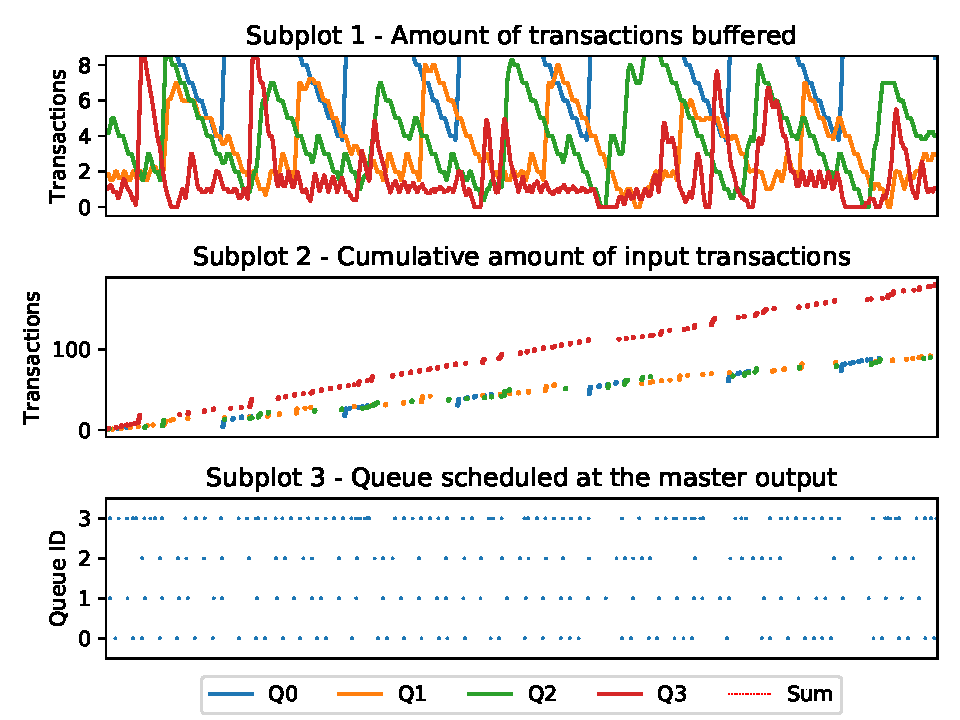
\includegraphics[scale=0.45]{images/SchIM_TS_buffering.pdf}
  %      \caption{TS with min. period of 160 clock cycles}
  %      \label{fig:schim_behaviour_mg}
        \textcolor{red}{TS subfigure removed}
      \end{subfigure}
      \caption{Trace snapshots of SchIM for FP (\ref{fig:schim_behaviour_fp}), TDMA (\ref{fig:schim_behaviour_tdma}) \removed{and TS (\ref{fig:schim_behaviour_mg})}}
      \label{fig:schim_behaviour}
    \end{figure}

\subsection{Memory Isolation}
\label{subsec:isolation}
To evaluate the capability of our \schim with respect to its ability to
ensure performance isolation between the cores, a set of experiments
involving SD-VBS benchmarks were designed. Here, we compare the
execution time of an application on a given core when running alone
(referred to as \emph{Solo}) and when running alongside interfering synthetic
benchmarks (write memory bombs) on all the other cores (referred to as
\emph{Stress}).
For each combination of a route to main memory (i.e., the \emph{normal
route} or the \emph{\schim route}) and scheduler, the result obtained
for \emph{Stress} is normalized with respect to the equivalent configuration
in \emph{Solo}.
%The slowdown compared to the case in which the observed
%benchmark runs alone in the system is computed while taking the same
%route to the main memory (i.e., the \emph{normal route} or the
%\empl{\schim route}).
%It follows that a ratio of 1 denotes the ideal isolation.
The results obtained on the considered benchmarks are listed in
Figure~\ref{fig:isolation_ratio}. All the results in the
Figure~\ref{fig:isolation_ratio} are the aggregation (arithmetic average)
of 30 different runs in the same configuration. Each bar cluster of the Figure~\ref{fig:isolation_ratio} insets represents one of the aforementioned configuration for \emph{Solo} and \emph{Stress}. The height of each bar denotes its normalized execution time.

For this set of experiments, the FP scheduler was configured such that the core under
analysis (i.e., the one running the benchmark) has the highest priority
and a threshold of 8. The other cores are assigned lower priorities and
thresholds matching their priority order (i.e., 4, 2, 1). Under TDMA scheduling, the core under analysis has a slot of 512 clock cycles and a threshold of 14 while the co-runners are assigned slots of 32 and 16 clock cycles with thresholds of 4 and 1.
\removed{
For the TS scheduler, the core under analysis is assigned a MIT of 16 and a threshold of 4 whereas each co-runner has a MIT of 64 and a threshold of 2.
}

The \emph{normal route} is used as a baseline for this experiment
because no scheduling is performed in this configuration.
%The results for
%the simple loop-back are displayed in the left-most column in
%Table~\ref{fig:isolation_ratio}.
The Figure \ref{fig:isolation_ratio} highlights the sensitivity of both
\emph{disparity} and \emph{mser} to inter-core interference on the
\emph{normal route}. This is especially the case for large input sizes
such as \emph{cif} and \emph{vga}. On the other hand, \emph{texture
synthesis} and \emph{localization} do not suffer from inter-core
interference.
Globally, the TDMA scheduler always manages to preserve the isolation of
the core, having execution times under \emph{Stress} similar or smaller than the \emph{normal route}. This is particularly visible for \emph{qcif}, \emph{cif} and \emph{vga} input sizes of \emph{disparity} and \emph{mser}.
%Unlike the \emph{normal route}, the TDMA scheduler manages to mitigate
%the impact of the inter-core interference on the core under analysis for
%\emph{disparity} and \emph{mser}. In fact, for \emph{qcif}, \emph{cif} and
%\emph{vga}, the scheduler is as good or better than the \emph{normal route}.
%In fact, the ratio of all the benchmarks we tested lie in
%the proximity of 1.0, with a maximum inter-core interference of around 7\%.
Similarly, the FP scheduler is also capable of ensuring sound
isolation of the core under analysis.
\removed{
Unfortunately, the TS scheduler generally fails to provide any form of
isolation. This is more than likely due to the logic defect mentioned in
Section \ref{subsec:internal-behaviour-of-schim}. In this case, the transaction leakage
prevents the transaction from the core under analysis to be served as they
unexpectedly occupy the bus, unpredictability delaying the scheduling of the other transactions.
}
% of the core under analysis
%despite having been assigned the highest priority. Even worst, the
%scheduler has a little-to-none impact since its slowdown is comparable
%to that observed on the loop-back path.
%This result can be explained by the fact that despite the enforcement of the FP policy, and its proven correct behavior (see \fig{fig:schim_behaviour_fp}), the
%This
%enforced ordering of transaction is likely overridden by the
%transaction re-ordering mechanisms present in the DDR controller. The
%problem specifically occurs because the access pattern of the
%interfering bombs is sequential, and hence preferably treated by the
%DDR controller. Conversely, the FP scheduler works correctly in
%scenarios like those in \fig{fig:schim_behaviour_fp} because the
%memory access pattern of the core under analysis is sequential as
%well. It follows that the FP policy is mainly useful when performing
%the movement of large, sequential data chunks.
\begin{figure}
    \centering
    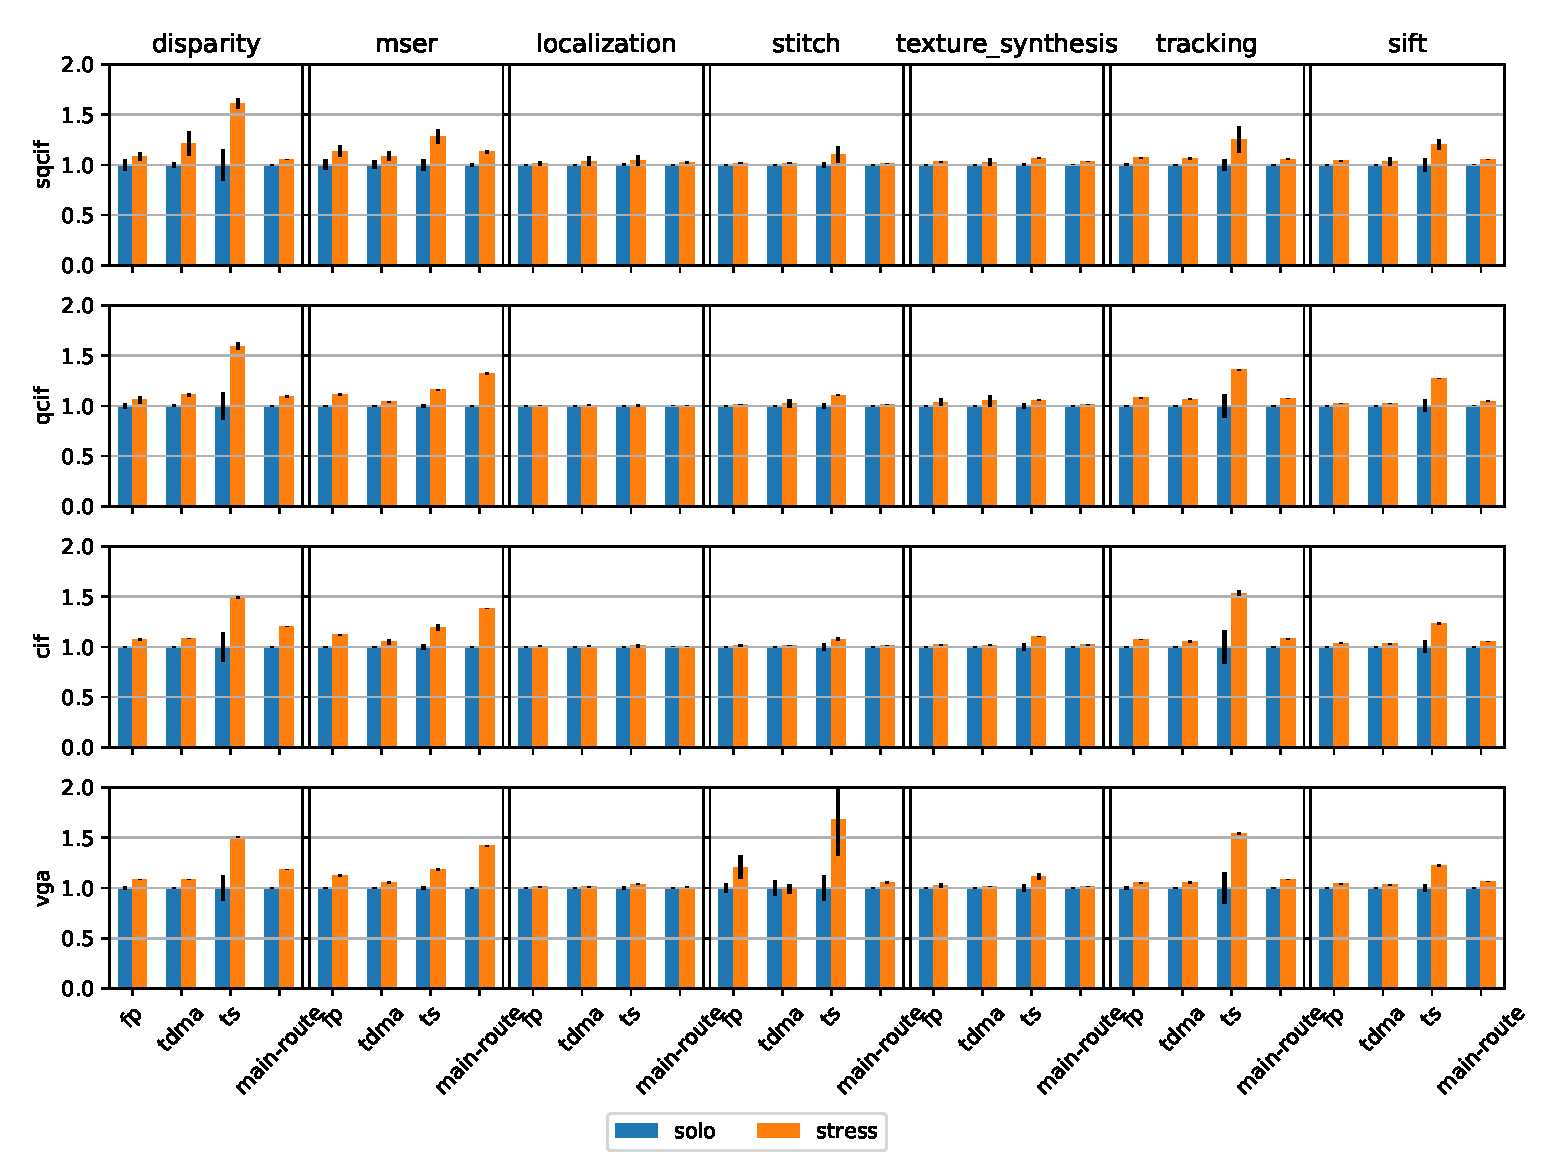
\includegraphics[scale=0.54]{images/Execution_times.pdf}
    \caption{Normalized execution time for each benchmark and input size for \emph{Solo} and \emph{Stress}. Each column denote a given benchmark of the SD-VBS suite, while each row denotes a specific input size (in increasing order from top to bottom).}
    \label{fig:isolation_ratio}
\end{figure}
